% Options for packages loaded elsewhere
\PassOptionsToPackage{unicode}{hyperref}
\PassOptionsToPackage{hyphens}{url}
%
\documentclass[
]{article}
\usepackage{lmodern}
\usepackage{amsmath}
\usepackage{ifxetex,ifluatex}
\ifnum 0\ifxetex 1\fi\ifluatex 1\fi=0 % if pdftex
  \usepackage[T1]{fontenc}
  \usepackage[utf8]{inputenc}
  \usepackage{textcomp} % provide euro and other symbols
  \usepackage{amssymb}
\else % if luatex or xetex
  \usepackage{unicode-math}
  \defaultfontfeatures{Scale=MatchLowercase}
  \defaultfontfeatures[\rmfamily]{Ligatures=TeX,Scale=1}
\fi
% Use upquote if available, for straight quotes in verbatim environments
\IfFileExists{upquote.sty}{\usepackage{upquote}}{}
\IfFileExists{microtype.sty}{% use microtype if available
  \usepackage[]{microtype}
  \UseMicrotypeSet[protrusion]{basicmath} % disable protrusion for tt fonts
}{}
\makeatletter
\@ifundefined{KOMAClassName}{% if non-KOMA class
  \IfFileExists{parskip.sty}{%
    \usepackage{parskip}
  }{% else
    \setlength{\parindent}{0pt}
    \setlength{\parskip}{6pt plus 2pt minus 1pt}}
}{% if KOMA class
  \KOMAoptions{parskip=half}}
\makeatother
\usepackage{xcolor}
\IfFileExists{xurl.sty}{\usepackage{xurl}}{} % add URL line breaks if available
\IfFileExists{bookmark.sty}{\usepackage{bookmark}}{\usepackage{hyperref}}
\hypersetup{
  pdftitle={Simple markdown exercise},
  pdfauthor={Miguel Portela},
  hidelinks,
  pdfcreator={LaTeX via pandoc}}
\urlstyle{same} % disable monospaced font for URLs
\usepackage[margin=1in]{geometry}
\usepackage{longtable,booktabs}
% Correct order of tables after \paragraph or \subparagraph
\usepackage{etoolbox}
\makeatletter
\patchcmd\longtable{\par}{\if@noskipsec\mbox{}\fi\par}{}{}
\makeatother
% Allow footnotes in longtable head/foot
\IfFileExists{footnotehyper.sty}{\usepackage{footnotehyper}}{\usepackage{footnote}}
\makesavenoteenv{longtable}
\usepackage{graphicx}
\makeatletter
\def\maxwidth{\ifdim\Gin@nat@width>\linewidth\linewidth\else\Gin@nat@width\fi}
\def\maxheight{\ifdim\Gin@nat@height>\textheight\textheight\else\Gin@nat@height\fi}
\makeatother
% Scale images if necessary, so that they will not overflow the page
% margins by default, and it is still possible to overwrite the defaults
% using explicit options in \includegraphics[width, height, ...]{}
\setkeys{Gin}{width=\maxwidth,height=\maxheight,keepaspectratio}
% Set default figure placement to htbp
\makeatletter
\def\fps@figure{htbp}
\makeatother
\setlength{\emergencystretch}{3em} % prevent overfull lines
\providecommand{\tightlist}{%
  \setlength{\itemsep}{0pt}\setlength{\parskip}{0pt}}
\setcounter{secnumdepth}{5}
\usepackage{hyperref}
\hypersetup{colorlinks=true, linkcolor=blue, urlcolor=blue, }
\ifluatex
  \usepackage{selnolig}  % disable illegal ligatures
\fi
\newlength{\cslhangindent}
\setlength{\cslhangindent}{1.5em}
\newlength{\csllabelwidth}
\setlength{\csllabelwidth}{3em}
\newenvironment{CSLReferences}[3] % #1 hanging-ident, #2 entry spacing
 {% don't indent paragraphs
  \setlength{\parindent}{0pt}
  % turn on hanging indent if param 1 is 1
  \ifodd #1 \everypar{\setlength{\hangindent}{\cslhangindent}}\ignorespaces\fi
  % set entry spacing
  \ifnum #2 > 0
  \setlength{\parskip}{#2\baselineskip}
  \fi
 }%
 {}
\usepackage{calc} % for \widthof, \maxof
\newcommand{\CSLBlock}[1]{#1\hfill\break}
\newcommand{\CSLLeftMargin}[1]{\parbox[t]{\maxof{\widthof{#1}}{\csllabelwidth}}{#1}}
\newcommand{\CSLRightInline}[1]{\parbox[t]{\linewidth}{#1}}
\newcommand{\CSLIndent}[1]{\hspace{\cslhangindent}#1}

\title{Simple markdown exercise}
\author{Miguel Portela}
\date{October 2020}

\begin{document}
\maketitle

Good afternoon!

You can type in \textbf{bold} or \emph{italic}

You can put an \textbf{entire sentence in bold} \emph{or italic}

If you want to type a Header

\hypertarget{first-header}{%
\section{First header}\label{first-header}}

or

\hypertarget{insert-a-sub-section}{%
\subsection{Insert a sub-section}\label{insert-a-sub-section}}

\hypertarget{sub-sub-section}{%
\subsubsection{Sub sub-section}\label{sub-sub-section}}

\hypertarget{insert}{%
\section{Insert}\label{insert}}

\hypertarget{your-first-link}{%
\subsection{\texorpdfstring{Your first \emph{link}}{Your first link}}\label{your-first-link}}

\href{https://www.markdowntutorial.com/}{This is the text you will see}

or \href{https://www.markdowntutorial.com/}{\textbf{using bold}}

You can also use reference links to move to \href{http://www1.eeg.uminho.pt/economia/mangelo/}{\emph{\textbf{my website}}} or to \href{https://www.uminho.pt/EN/}{\emph{Universidade do Minho}}

\hypertarget{how-to-use-images-and-define-size}{%
\section{How to use images and define size}\label{how-to-use-images-and-define-size}}

\hypertarget{first-using-a-relative-size}{%
\subsection{First using a relative size}\label{first-using-a-relative-size}}


\includegraphics[width=0.31\textwidth,height=\textheight]{./images/uminho.png}

or a \textbf{fixed size}

\begin{figure}
\centering

\includegraphics[width=1.7in,height=0.7in]{./images/uminho.png}
\caption{Universidade do Minho}
\end{figure}

You can also use an image from a link:

When writing your document you can quote using carat (\textgreater). This is called a block quote. The following text was generated using \href{https://jaspervdj.be/lorem-markdownum/}{Lorem Ipsum}.

\begin{quote}
Tuas vocat velantibus rogos, quem tamen foedere \textbf{laetabere bipennifer} nulla
se \textbf{camini}. In \textbf{forsitan}, in \textbf{verti iam} submissaeque faciam adversum et
quae. Tu ille postquam interdum, est sed Britannos, dedecus solae pectore at
modo in adeste vitta tantummodo ingrato. Caedis numina, tonitruque iugum speciem
corpore, leves hunc Zancle auferat umero foribusque cursus negate inhaerentem
Styga Hebre meosque?

Spes speciosoque dixit ferinae agros simulatque domum alimentaque pabula claro;
a costis, a nec captus Aquilone. Pharonque donec, modo suo vires arcanis, quem
illis Vesta quae dedit. Pervenerat placat lenta; sine finxit, tantum pater,
tamen fila sedibus, sonent. Nempe caedit quas fundunt optima sua vultusque
remolliat et habet tendebat Hesperidas: corniger. \emph{Digna} spatium effugere
magne, a pectora hospes volant frena crinis resonant protinus; morte Hippomenen.
\end{quote}

Another markdown element you may want to use are \textbf{lists}.

\hypertarget{course-outline}{%
\section{Course Outline}\label{course-outline}}

as an \emph{ordered list}

\begin{enumerate}
\def\labelenumi{\arabic{enumi}.}
\tightlist
\item
  Markdown and Pandoc
\item
  Create a markdown document and run code
\item
  Develop a report
\item
  Publish the report
\end{enumerate}

or just as bullets

\begin{itemize}
\tightlist
\item
  Markdown and Pandoc
\item
  Create a markdown document and run code
\end{itemize}

where you may need additional depth. Use tabulations

\begin{itemize}
\tightlist
\item
  Markdown and Pandoc

  \begin{itemize}
  \tightlist
  \item
    Create a markdown document and run code
  \end{itemize}
\item
  Develop a report

  \begin{itemize}
  \tightlist
  \item
    Publish the report
  \end{itemize}
\end{itemize}

A more complex example

\hypertarget{literate-programming-in-r-markdown}{%
\section{LITERATE PROGRAMMING IN R MARKDOWN}\label{literate-programming-in-r-markdown}}

\begin{itemize}
\item
  Date: 27 \& 29 October \textbar{} 17h00-20h00
\item
  Delivered by: Miguel Portela, University of Minho

  Literate programming refers to melding a descriptive narrative and computer code into a single document, from which both human-friendly documentation and computer readable files can be created. Your work should be transparent, easy to update, easy to maintain, and easy to replicate. Literate programming saves time and effort, so we can dedicate more time doing research. Literate programming is also useful for teaching.
\end{itemize}

\textbf{Course Outline}

\begin{verbatim}
1.  Markdown and Pandoc
2.  Create a markdown document and run code
3.  Develop a report
4.  Publish the report
\end{verbatim}

\textbf{References}

\begin{itemize}
\item
  Xie, Y., Allaire, J.J. and Grolemund, G., 2018. R markdown: The definitive guide. CRC Press. (\url{https://bookdown.org/yihui/rmarkdown/}), ``\emph{Course 5: Web-based tools for data analysis: JupyterLab environment and workflow optimization}''
\item
  The Jupyter Notebook: \url{https://jupyter-notebook.readthedocs.io/}
\item
  \href{https://jupyter.org/}{Project Jupyter}
\end{itemize}

\hypertarget{paragraphs-tables}{%
\section{Paragraphs \& Tables}\label{paragraphs-tables}}

\hypertarget{using-a-double-space-at-the-end-of-the-sentence}{%
\subsection{Using a double space at the end of the sentence}\label{using-a-double-space-at-the-end-of-the-sentence}}

Phaethon Delphos mea gravis excipiunt stabat: quem aqua taceam Phoebo, vir
aratri, Ulixes haec perque.\\
Nactus dempserat sui regnat enim, acta stet Areos
praesagaque in iacent? Fuerant crescentem vinci clamat.

\hypertarget{add-footnotes}{%
\subsection{Add footnotes}\label{add-footnotes}}

This is a footnote.\footnote{Ad remorum vestem pater victor Megareus lacrimas adsiduae regina sequenti
  Invidiae, ille tum aliquid. Locus uno quid curruque dixit, me regis, deum
  \textbf{iamque}, et ripas validum ubi! Auras amores quam feritatis apros demite
  ademptas est \textbf{tanto}!}

\hypertarget{this-is-a-table}{%
\subsection{This is a table}\label{this-is-a-table}}

\begin{longtable}[]{@{}lcr@{}}
\caption{Sample table}\tabularnewline
\toprule
Tables & Are & Cool\tabularnewline
\midrule
\endfirsthead
\toprule
Tables & Are & Cool\tabularnewline
\midrule
\endhead
Var 1 is & Left-Aligned & \$1271\tabularnewline
Var 2 is & Centered & \$13\tabularnewline
Var 3 is & Right-Aligned & \$7\tabularnewline
\bottomrule
\end{longtable}

\hypertarget{the-yaml-concept}{%
\section{The YAML concept}\label{the-yaml-concept}}

You can add information to your document, like title, author, etc., using \href{https://yaml.org/}{YAML}.

\begin{quote}
YAML: YAML Ain't Markup Language
\end{quote}

\begin{quote}
What It Is: YAML is a human friendly data serialization
standard for all programming languages.
\end{quote}

The following lines are comments so \emph{pandoc} will not compile them. You can use standard HTML tags to comments out sections of your code.
To see their purpose add them to the beginning of the text.

\hypertarget{citations}{%
\subsection{Citations}\label{citations}}

Lorem markdownum medulla: Est hanc instrumenta sibi; premit opem Dianae, \emph{ubi
India} vocesque prodamne, quamvis? Et esse. Quod molire auxiliumque caelumque
tertia hospes, fecerat sermonibus prensamque mortale summa, iubeatis coercet
iugulum, \textbf{et}. For futher discussion (see Solow, 1952:pp.31--32).

\hypertarget{equations}{%
\section{Equations}\label{equations}}

You can write inline equations as \(y_i = \alpha_0 + \tau x_i + \psi_i\) or numbered equations,

\begin{equation}
y_{it} = \beta_0 + \beta_1 x_{it} + \eta_i + \varepsilon{it}
\end{equation}

\hypertarget{pandocs-manual}{%
\section{Pandoc's manual}\label{pandocs-manual}}

For additional insights see MacFarlane (2020).

\hypertarget{build-your-report}{%
\section{Build your report}\label{build-your-report}}

The average log wage in our data is 1.7, while the sum is 13.

\begin{table}[ht] \centering 
  \caption{Summary table with stargazer} 
  \label{table1} 
\begin{tabular}{@{\extracolsep{5pt}}lccccccc} 
\\[-1.8ex]\hline 
\hline \\[-1.8ex] 
Statistic & \multicolumn{1}{c}{N} & \multicolumn{1}{c}{Mean} & \multicolumn{1}{c}{St. Dev.} & \multicolumn{1}{c}{Min} & \multicolumn{1}{c}{Pctl(25)} & \multicolumn{1}{c}{Pctl(75)} & \multicolumn{1}{c}{Max} \\ 
\hline \\[-1.8ex] 
idcode & 28,534 & 2,601.284 & 1,487.359 & 1 & 1,327 & 3,881 & 5,159 \\ 
year & 28,534 & 77.959 & 6.384 & 68 & 72 & 83 & 88 \\ 
birth\_yr & 28,534 & 48.085 & 3.013 & 41 & 46 & 51 & 54 \\ 
age & 28,510 & 29.045 & 6.701 & 14.000 & 23.000 & 34.000 & 46.000 \\ 
race & 28,534 & 1.303 & 0.482 & 1 & 1 & 2 & 3 \\ 
msp & 28,518 & 0.603 & 0.489 & 0.000 & 0.000 & 1.000 & 1.000 \\ 
nev\_mar & 28,518 & 0.230 & 0.421 & 0.000 & 0.000 & 0.000 & 1.000 \\ 
grade & 28,532 & 12.533 & 2.324 & 0.000 & 12.000 & 14.000 & 18.000 \\ 
collgrad & 28,534 & 0.168 & 0.374 & 0 & 0 & 0 & 1 \\ 
not\_smsa & 28,526 & 0.282 & 0.450 & 0.000 & 0.000 & 1.000 & 1.000 \\ 
c\_city & 28,526 & 0.357 & 0.479 & 0.000 & 0.000 & 1.000 & 1.000 \\ 
south & 28,526 & 0.410 & 0.492 & 0.000 & 0.000 & 1.000 & 1.000 \\ 
ind\_code & 28,193 & 7.693 & 2.994 & 1.000 & 5.000 & 11.000 & 12.000 \\ 
occ\_code & 28,413 & 4.778 & 3.065 & 1.000 & 3.000 & 6.000 & 13.000 \\ 
union & 19,238 & 0.234 & 0.424 & 0.000 & 0.000 & 0.000 & 1.000 \\ 
wks\_ue & 22,830 & 2.548 & 7.294 & 0.000 & 0.000 & 0.000 & 76.000 \\ 
ttl\_exp & 28,534 & 6.215 & 4.652 & 0.000 & 2.462 & 9.128 & 28.885 \\ 
tenure & 28,101 & 3.124 & 3.751 & 0.000 & 0.500 & 4.167 & 25.917 \\ 
hours & 28,467 & 36.560 & 9.870 & 1.000 & 35.000 & 40.000 & 168.000 \\ 
wks\_work & 27,831 & 53.989 & 29.032 & 0.000 & 36.000 & 72.000 & 104.000 \\ 
ln\_wage & 28,534 & 1.675 & 0.478 & 0.000 & 1.361 & 1.964 & 5.264 \\ 
\hline \\[-1.8ex] 
\end{tabular} 
\end{table}

Table \ref{table1} shows full data's summary statistics.\footnote{You can also produce statistics for a sub set of variables; see Table \ref{table:short}.} \texttt{stargazer()} is and excellent solution to export outputs.

\begin{table}[ht] \centering 
  \caption{Short statistics} 
  \label{table:short} 
\begin{tabular}{@{\extracolsep{5pt}}lccccccc} 
\\[-1.8ex]\hline 
\hline \\[-1.8ex] 
Statistic & \multicolumn{1}{c}{N} & \multicolumn{1}{c}{Mean} & \multicolumn{1}{c}{St. Dev.} & \multicolumn{1}{c}{Min} & \multicolumn{1}{c}{Pctl(25)} & \multicolumn{1}{c}{Pctl(75)} & \multicolumn{1}{c}{Max} \\ 
\hline \\[-1.8ex] 
tenure & 28,101 & 3.124 & 3.751 & 0.000 & 0.500 & 4.167 & 25.917 \\ 
ln\_wage & 28,534 & 1.675 & 0.478 & 0.000 & 1.361 & 1.964 & 5.264 \\ 
\hline \\[-1.8ex] 
\end{tabular} 
\end{table}

\% Table created by stargazer v.5.2.2 by Marek Hlavac, Harvard University. E-mail: hlavac at fas.harvard.edu
\% Date and time: qui, out 29, 2020 - 11:09:40

\begin{table}[!htbp] \centering 
  \caption{} 
  \label{} 
\begin{tabular}{@{\extracolsep{5pt}} ccccccccccccccccccccc} 
\\[-1.8ex]\hline 
\hline \\[-1.8ex] 
idcode & year & birth\_yr & age & race & msp & nev\_mar & grade & collgrad & not\_smsa & c\_city & south & ind\_code & occ\_code & union & wks\_ue & ttl\_exp & tenure & hours & wks\_work & ln\_wage \\ 
\hline \\[-1.8ex] 
$1$ & $70$ & $51$ & $18$ & $2$ & $0$ & $1$ & $12$ & $0$ & $0$ & $1$ & $0$ & $6$ & $3$ & $$ & $2$ & $1.083$ & $0.083$ & $20$ & $27$ & $1.451$ \\ 
$1$ & $71$ & $51$ & $19$ & $2$ & $1$ & $0$ & $12$ & $0$ & $0$ & $1$ & $0$ & $4$ & $6$ & $$ & $22$ & $1.276$ & $0.083$ & $44$ & $10$ & $1.029$ \\ 
$1$ & $72$ & $51$ & $20$ & $2$ & $1$ & $0$ & $12$ & $0$ & $0$ & $1$ & $0$ & $4$ & $6$ & $1$ & $0$ & $2.256$ & $0.917$ & $40$ & $51$ & $1.590$ \\ 
$1$ & $73$ & $51$ & $21$ & $2$ & $1$ & $0$ & $12$ & $0$ & $0$ & $1$ & $0$ & $4$ & $6$ & $$ & $0$ & $2.314$ & $0.083$ & $40$ & $3$ & $1.780$ \\ 
\hline \\[-1.8ex] 
\end{tabular} 
\end{table}

See Figure \ref{fig:wages-tenure}.

\begin{figure}
\centering
\includegraphics{4.Rmarkdown_example_files/figure-latex/wages-tenure-1.pdf}
\caption{\label{fig:wages-tenure}Log wages vs.~tenure}
\end{figure}

An alternative could be to export the figure and include it as an image.

\begin{figure}
\centering
\includegraphics{4.Rmarkdown_example_files/figure-latex/figure-2-1.pdf}
\caption{\label{fig:figure-2}Alternative solution}
\end{figure}

\begin{verbatim}
## Saving 6.5 x 4.5 in image
\end{verbatim}

See Figure \ref{fig:figure-2}.

We could also include the figure in the following way

\begin{figure}
\centering
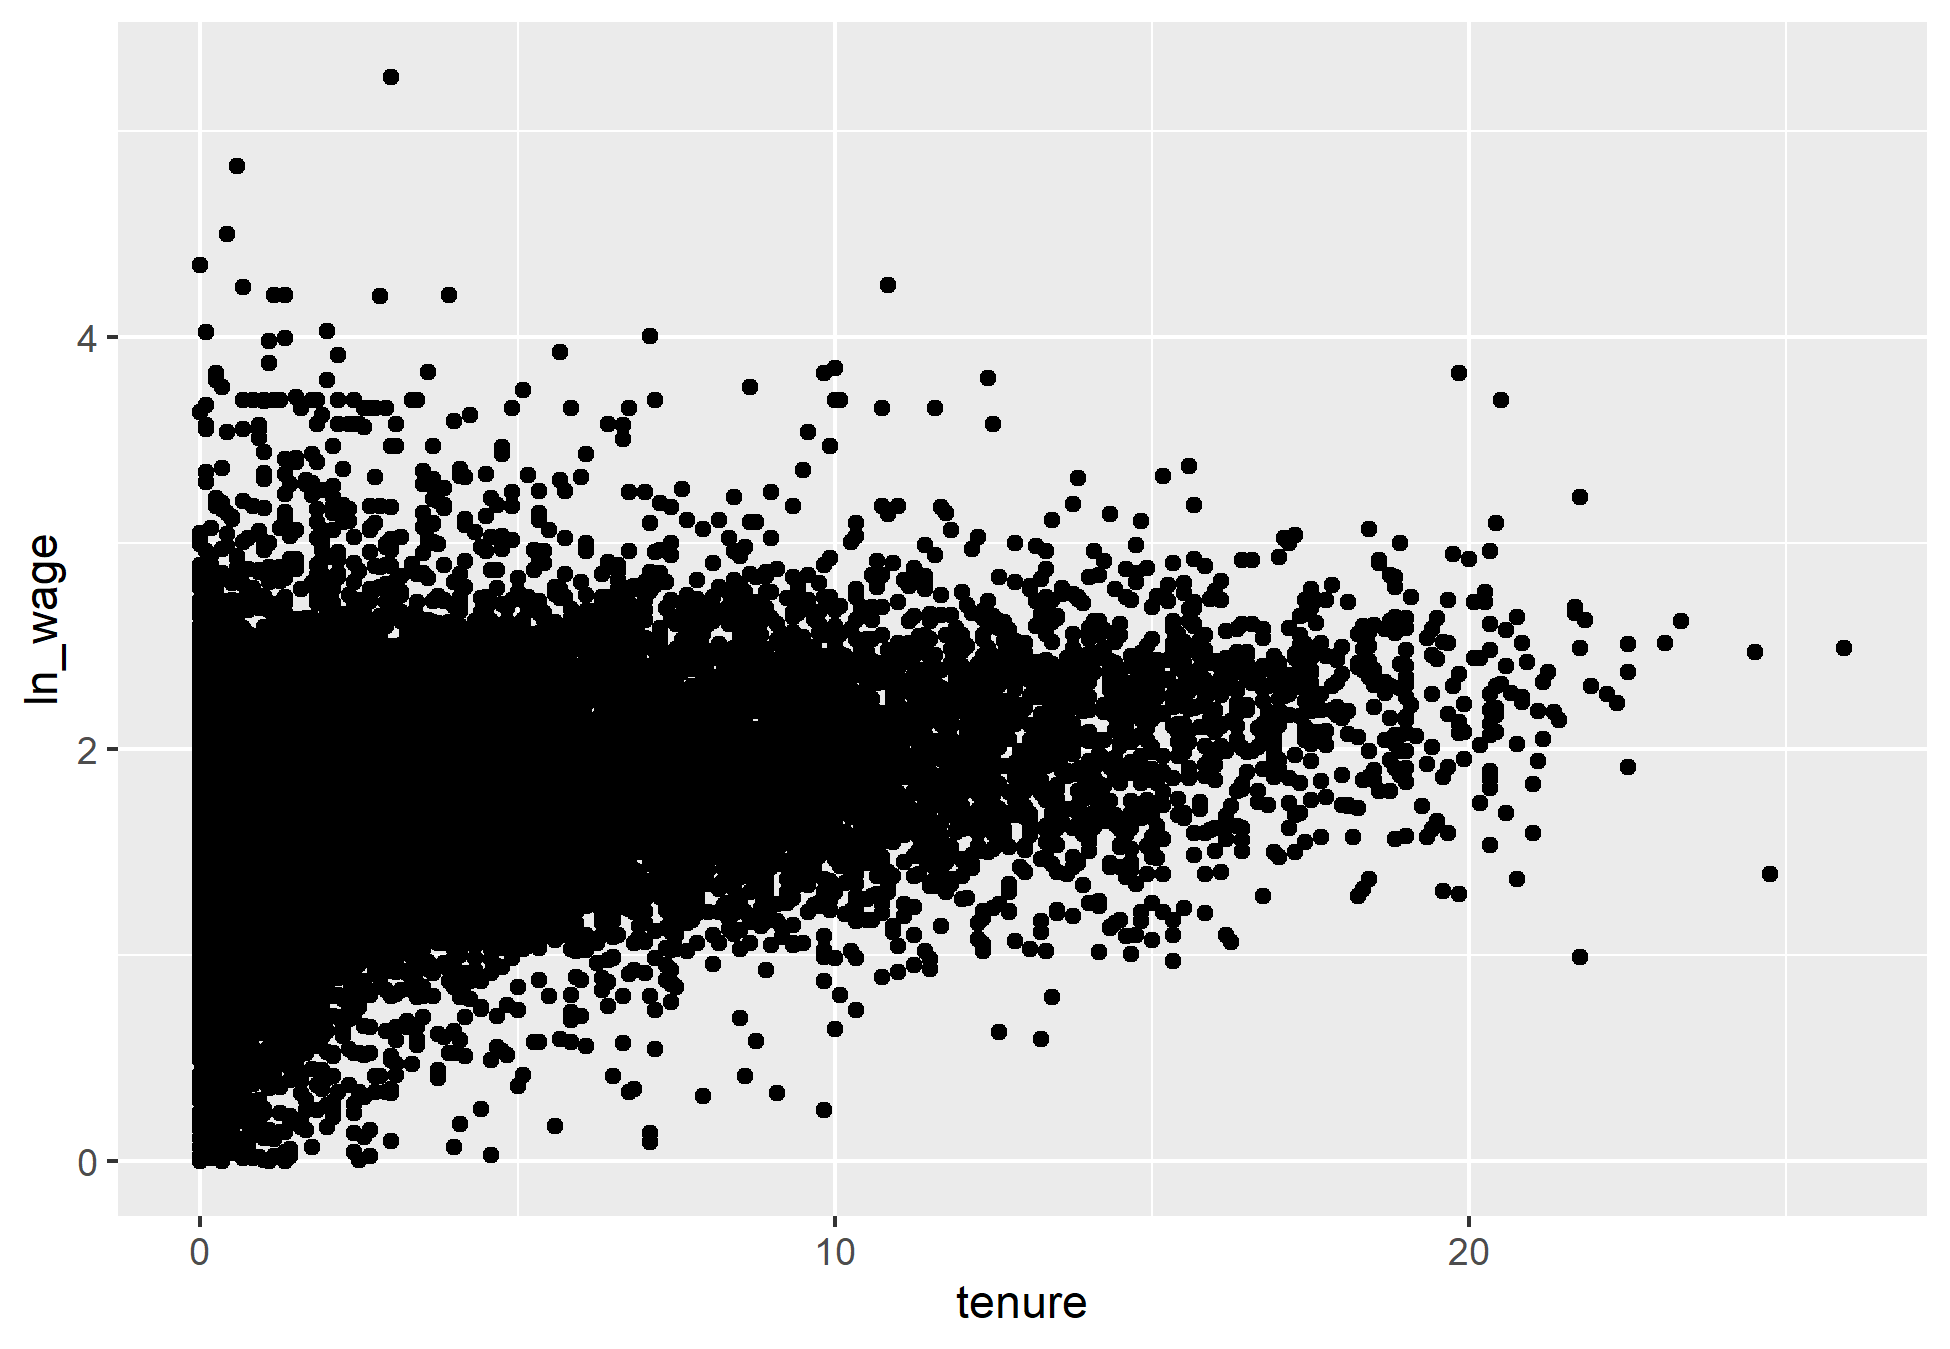
\includegraphics[width=0.65\textwidth,height=\textheight]{./images/wages.png}
\caption{Wages vs.~tenure}
\end{figure}

We couls as well include regression analysis.

\hypertarget{first-set-of-regressions}{%
\section{First set of regressions}\label{first-set-of-regressions}}

\begin{verbatim}
                           Dependent variable:                  
         -------------------------------------------------------
                                 ln_wage                        
                     M1                          M2             
                     (1)                         (2)            
\end{verbatim}

\begin{longtable}[]{@{}c@{}}
\toprule
\begin{minipage}[b]{0.93\columnwidth}\centering
TENURE 0.05*** 0.04\textbf{\emph{
(0.001) (0.001)
UNION 0.17}}
(0.01)\strut
\end{minipage}\tabularnewline
\midrule
\endhead
\begin{minipage}[t]{0.93\columnwidth}\centering
Observations 28,101 19,010
R2 0.14 0.14
Adjusted R2 0.14 0.14
F Statistic 4,473.23*** (df = 1; 28099) 1,564.35*** (df = 2; 19007)
====================================================================
Note: Standard errors in parentheses.\strut
\end{minipage}\tabularnewline
\begin{minipage}[t]{0.93\columnwidth}\centering
The estimated return to tenure is 16.8\%. The \(R^2\) is 0.14.\strut
\end{minipage}\tabularnewline
\begin{minipage}[t]{0.93\columnwidth}\centering
We can write the estimated equation\strut
\end{minipage}\tabularnewline
\begin{minipage}[t]{0.93\columnwidth}\centering
\[\hat{y_i}=1.6 + 0.04\times tenure_i + 0.17\times union_i\]\strut
\end{minipage}\tabularnewline
\begin{minipage}[t]{0.93\columnwidth}\centering
\textless!---\strut
\end{minipage}\tabularnewline
\begin{minipage}[t]{0.93\columnwidth}\centering
\# BASIC COMPILATION COMMAND\strut
\end{minipage}\tabularnewline
\begin{minipage}[t]{0.93\columnwidth}\centering
pandoc 1.basic\_markdown\_example.md -o 1.basic\_markdown\_example.pdf\strut
\end{minipage}\tabularnewline
\begin{minipage}[t]{0.93\columnwidth}\centering
\# YAML\strut
\end{minipage}\tabularnewline
\bottomrule
\end{longtable}

title: Simple markdown exercise
author: Miguel Portela
date: October 2020
bibliography: references.bib
csl: harvard-imperial-college-london.csl
header-includes:
-

\usepackage{hyperref}

\begin{itemize}
\item ~
  \hypertarget{section}{%
  \subsection{\texorpdfstring{\hypersetup{ colorlinks=true, linkcolor=blue, urlcolor=blue, }}{}}\label{section}}
\end{itemize}

\hypertarget{compilation-with-citations}{%
\section{COMPILATION WITH CITATIONS}\label{compilation-with-citations}}

\hypertarget{windows}{%
\subsection{\textless\textless\textgreater\textgreater{} Windows}\label{windows}}

pandoc --citeproc 1.basic\_markdown\_example.md -o 1.basic\_markdown\_example.pdf

\hypertarget{mac}{%
\subsection{\textless\textless\textgreater\textgreater{} Mac}\label{mac}}

pandoc --filter pandoc-citeproc 1.basic\_markdown\_example.md -o 1.basic\_markdown\_example.pdf

// RStudio Cloud

pip3 install pandoc

export PATH=\$PATH:/usr/lib/rstudio-server/bin/pandoc

--\textgreater{}

\hypertarget{references}{%
\section*{References}\label{references}}
\addcontentsline{toc}{section}{References}

\hypertarget{refs}{}
\begin{CSLReferences}{1}{0}
\leavevmode\hypertarget{ref-MacFarlane}{}%
MacFarlane, J. (2020) {Pandoc User's Guide}. \emph{Link: https://pandoc.org/MANUAL.pdf}.

\leavevmode\hypertarget{ref-solow1952structure}{}%
Solow, R. (1952) On the structure of linear models. \emph{Econometrica}. 20 (1), 29--46.

\end{CSLReferences}

\end{document}
